% Chapter3

\chapter{Preliminary Design} % Main chapter title

\label{Chapter3} % For referencing the chapter elsewhere, use \ref{Chapter1} 

\lhead{Chapter 3. \emph{Preliminary Design}} % This is for the header on each page - perhaps a shortened title

%----------------------------------------------------------------------------------------
\section{Design Specification}
\subsection{Major Functions}
There are four major functions of the senior community center project:
\begin{enumerate}
\item Providing housing units to elder population in the surrounding
  communities and newly enrolled faculty members. Providing choices of 
  various degrees of care and the special care of Aalzheimer's
  disease. 
\item As a result of the collaboration with the OSHER (Lifelone
  Learning Center), providing classrooms and administrative officies
  for OSHER. 
\item Providing labs for aging related researches.
\item Create common space for inter-generation activities
\end{enumerate}

\clearpage
\section{Site Planning}
The site plan of the building consider to create a bridge between the
senior center and the parking garage. The major goal of this bridge is
to provide the children and elderly a safe way of crossing the Forbes
Ave. between the main campus and the proposed site. An entrance facing
east is also provided on the third floor of the senior center. The
anticipation for this design choice is that the student from the
Doherty Apartment can use the public space on the third floor and the
bridge to cross the Forbes Ave~\fref{fig:bridge}.~
\begin{figure}[h!]
\centering
\begin{subfigure}{0.6\textwidth}
  \centering
  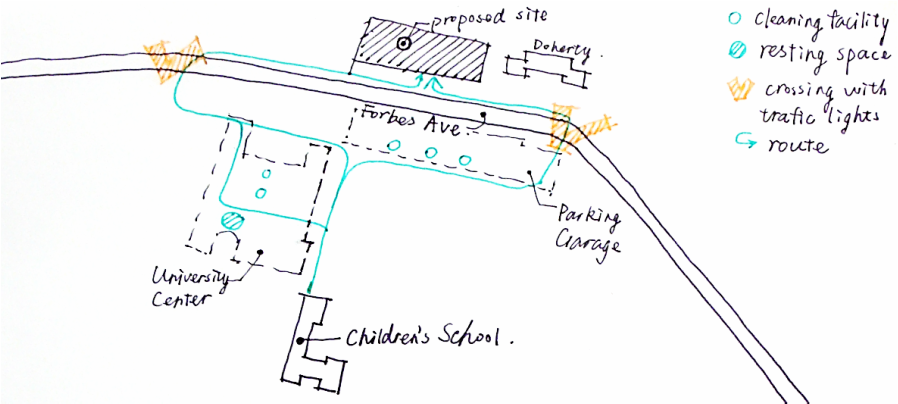
\includegraphics[width=\linewidth]{bridge1.png}
  \caption{Detouring Path from Children's School to the Proposed Site}
  \label{fig:bridge1}
\end{subfigure}
\begin{subfigure}{0.6\textwidth}
  \centering
  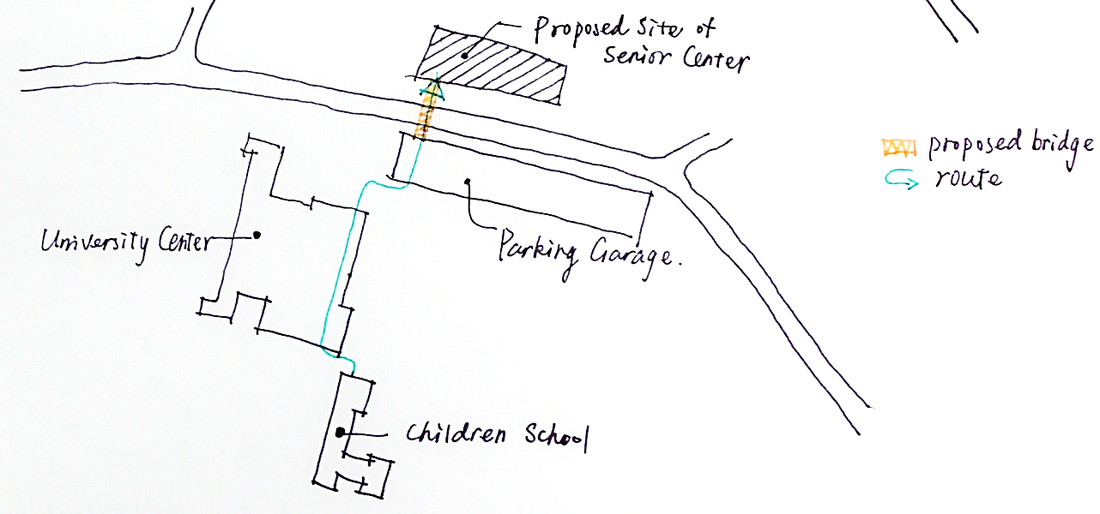
\includegraphics[width=\linewidth]{bridge2.png}
  \caption{Creating a Bridge to Reduce Detouring Distance}
  \label{fig:bridge2}
\end{subfigure}
\caption{Bridge Connecting Parking Garage and Senior Center}
\label{fig:bridge}
\end{figure}

\clearpage
\begin{figure}
\centering
\begin{subfigure}{\textwidth}
  \centering
  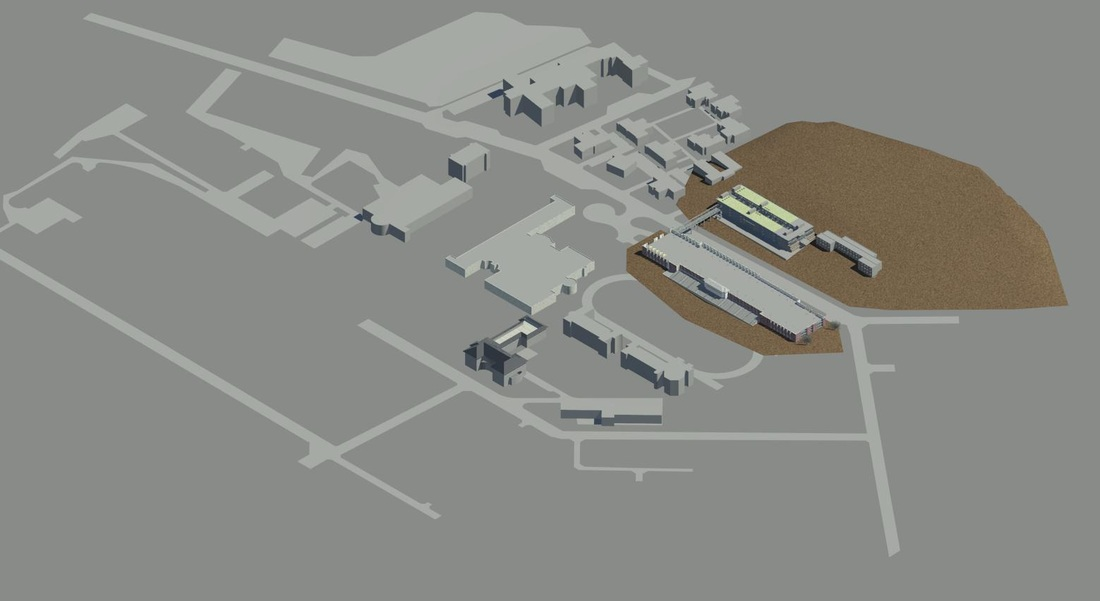
\includegraphics[width=0.8\textwidth]{site.jpg}
  \caption[Site Planning]{Site Planning Perspective View}
  \label{fig:site}
\end{subfigure}
\begin{subfigure}{\textwidth}
  \centering
  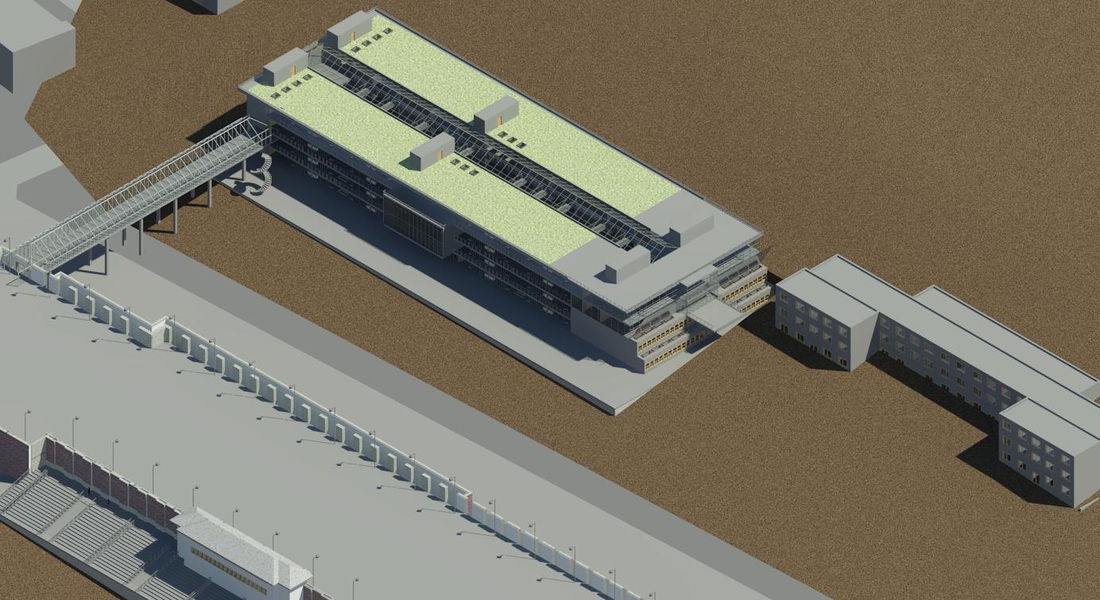
\includegraphics[width=0.8\textwidth]{siteClose.jpg}
  \caption[Site Planning Closer View]{Site Planning Closer View}
  \label{fig:siteClose}
\end{subfigure}
\caption{Site Planning}
\label{fig:siteAll}
\end{figure}

\clearpage
By this design choice, an intersection of routes are created for the
elderly, the children and the young students, providing the
opportunity for inter-generation connection. Thus a ``public living
room'' was arranged on the top floor in the form of a cafe and some
crafts room. ~
\begin{figure}[h!]
  \centering
  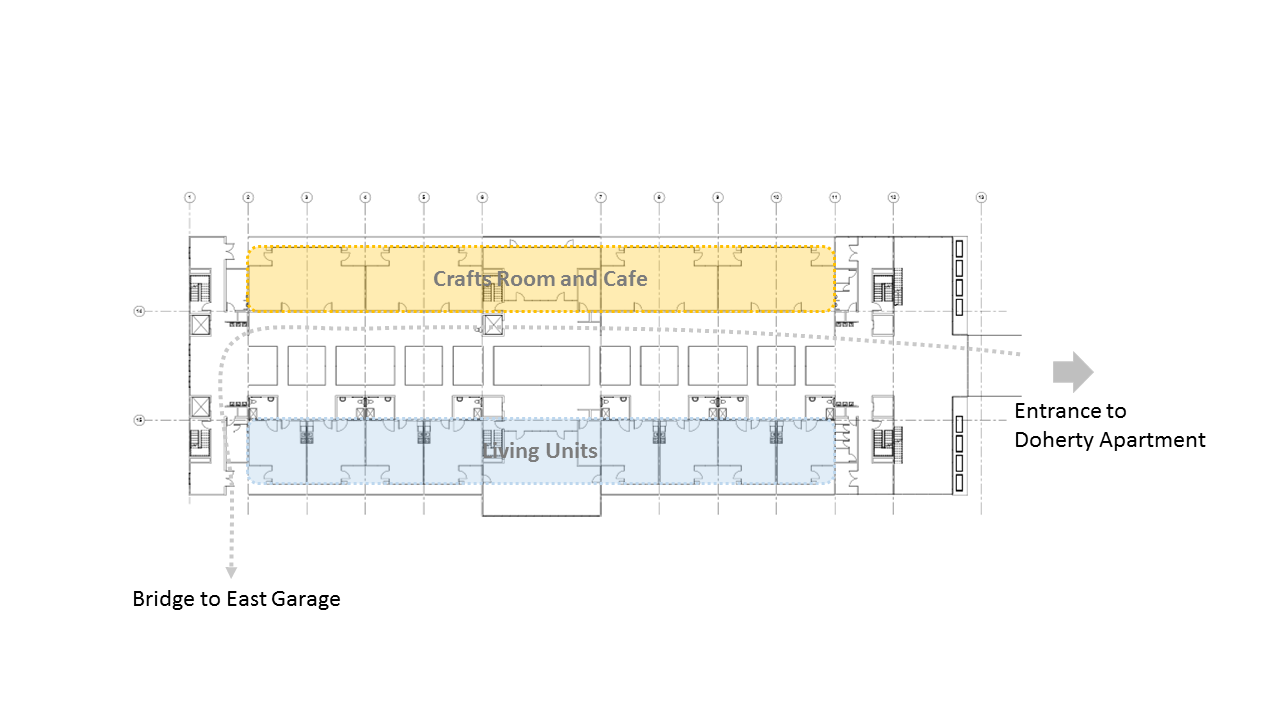
\includegraphics[width=\textwidth]{pathToD.png}
  \caption[Common Space on Third Floor Entrance]{Common Space on Third
    Floor}
  \label{fig:pathToD}
\end{figure}

\clearpage
\section{Living Unit and Group Design}
\subsection{Topological Pattern of Living Cluster Design}
There are two aspects of aging: the ``biological process'' and the
``social passage''. For the social passage, as one become aged, one
tends to encounter a dramatic change in the social roles, some tends
to withdraw from previous responsibilities, some seeks to engagement
in new social roles~\cite{Perkins2004}. Providing a soft transition
and a variety of choices is a key to maintain a balance between the
social connection and the degree of privacy. 

Also from the case study section, one of the key components for
Alzheimer's Care is to create a hierarchical public space. Upon the
concern of both of the two aspect, the basic space structure of
public-private-transition is defined recursively as depicted in
\fref{fig:spacePrivacy}.~
\begin{figure}[h!]
\centering
\begin{subfigure}{0.7\textwidth}
  \centering
  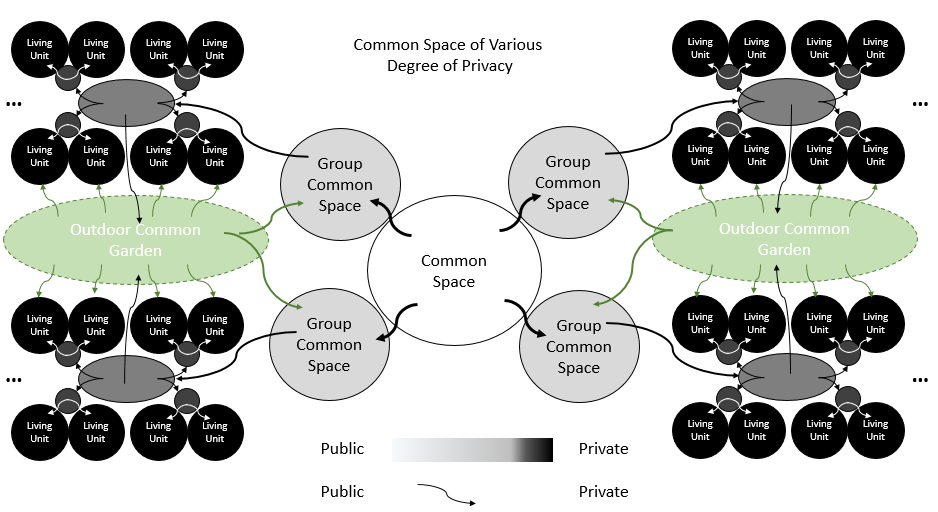
\includegraphics[width=\linewidth]{spacePattern.png}
  \caption{Space Pattern: Soft Transition of Public and Private Space}
  \label{fig:spacePattern}
\end{subfigure}
\begin{subfigure}{0.7\textwidth}
  \centering
  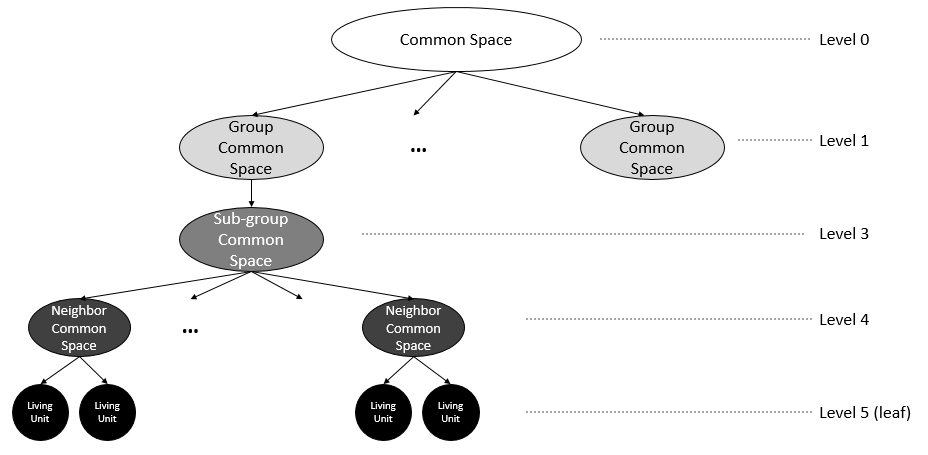
\includegraphics[width=\linewidth]{spaceTree.png}
  \caption{Tree Representation of Degree of Privacy Level}
  \label{fig:spaceTree}
\end{subfigure}
\caption{Space Pattern of Privacy Level Transition}
\label{fig:spacePrivacy}
\end{figure}

One reason to organize space in this pattern is to encourage a
group-assist living pattern, to encourage residents to give and
receive help from their neighbors and the living group, which can both
provide a sense of self-achievement for helping others, to prolong the
time of transferring to a higher nursing degree and to strengthen
bounds between residents. Since the housing project can also provide
housing unit to newly enrolled faculty members, the providing and
receiving of aids could also facilitate the inter-generation
connection.

Another concern is the varied degree layout facilitates privacy in
care-giving and receiving with small nursing group. This provides the
basis for creating a wide range of choices of different level of care.

Yet another consideration is to assign each group a common space and
encourage the residents to arrange the decoration and space
functionality, which increases the sense of belonging and also
provides Alzheimer victims with more clues for way finding.

\clearpage
\subsection{Design Living Unit}~
The living unit include a living and bedroom (452 sq.ft.), a bath room
(88 sq.ft) and a balcony. The living room includes cooking facility.
The design of living units account for the easiness for the turning
over of wheel chair, so the room layout does not contain hard
partition, which also take into consideration the in-room wandering
path that concerns Alzheimer's disease victims (\fref{fig:plan1unit}).~
\begin{figure}[h!]
  \centering
  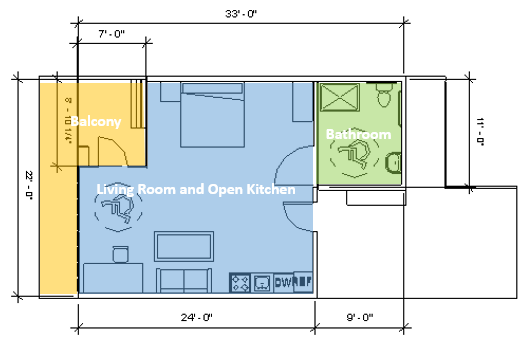
\includegraphics[width=0.7\textwidth]{plan1unit.png}
  \caption[Plan of Living Unit]{Plan of Living Unit}
  \label{fig:plan1unit}
\end{figure}
~
\begin{figure}[htbp]
  \centering
  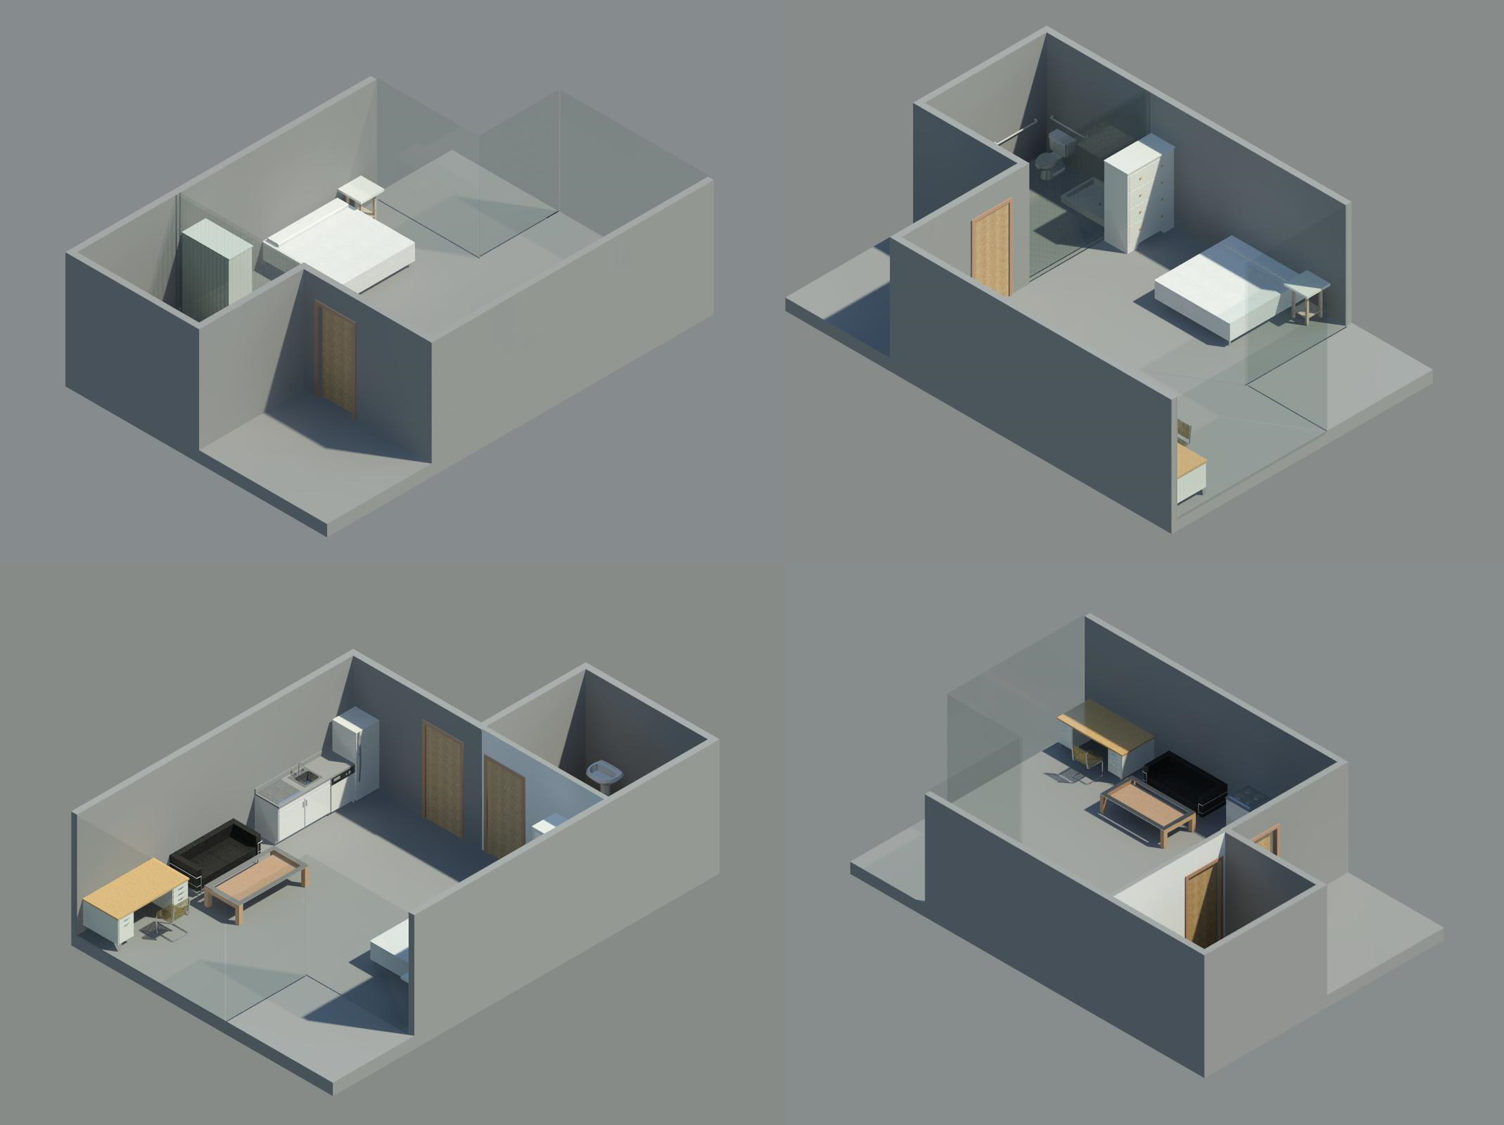
\includegraphics[width=\textwidth]{persUnit.png}
  \caption[Perspective View of Living Unit]{Perspective View of Living
    Unit}
  \label{fig:persUnit}
\end{figure}

Two adjacent living unit could be combined to for a single two-bedroom
two-bathroom living unit (\fref{fig:plan2unit}). This arrangement
can adapt to elderly couples (\fref{fig:plan2unit}).~
\begin{figure}[h!]
  \centering
  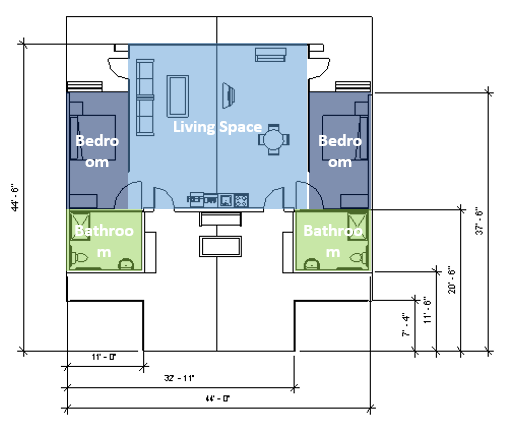
\includegraphics[width=0.7\textwidth]{plan2unit.png}
  \caption[Plan of Two-Unit Group]{Plan of Two-Unit Group}
  \label{fig:plan2unit}
\end{figure}
\begin{figure}[htbp]
  \centering
  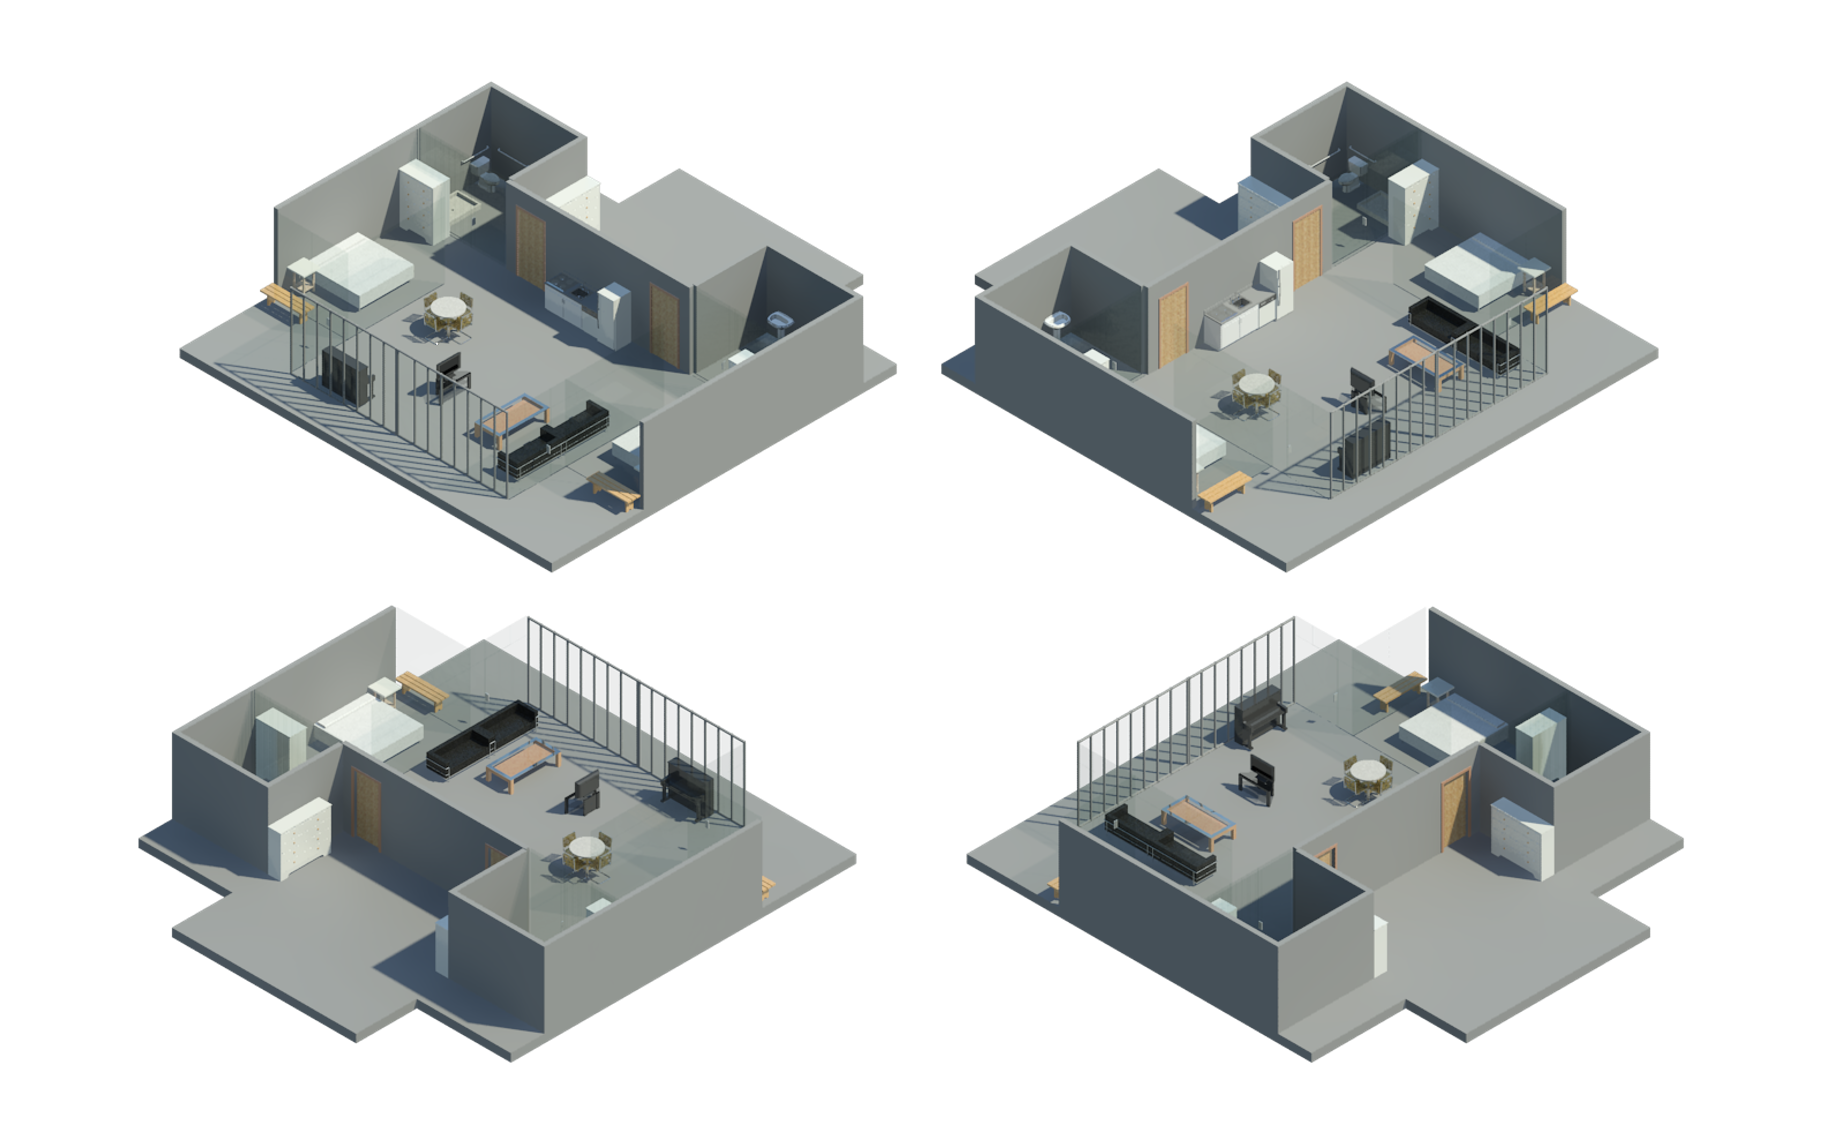
\includegraphics[width=\textwidth]{pers2unit.png}
  \caption[Perspective View of Two-Unit Group]{Perspective View of
    Two-Unit Group}
  \label{fig:pers2unit}
\end{figure}

\subsection{Common Space between Living Unit}
A concave space in front of the entrance of the adjacent two unit
defines a common entrance of the two neighboring units. Residents can
customize the layout and arrangement of the common space
together. This common space act as the bottom level of the
hierarchical public-private space transition
({fig:twoUnitCommonSpaceEntrance}).~
\begin{figure}[h!]
\centering
\begin{subfigure}{\textwidth}
  \centering
  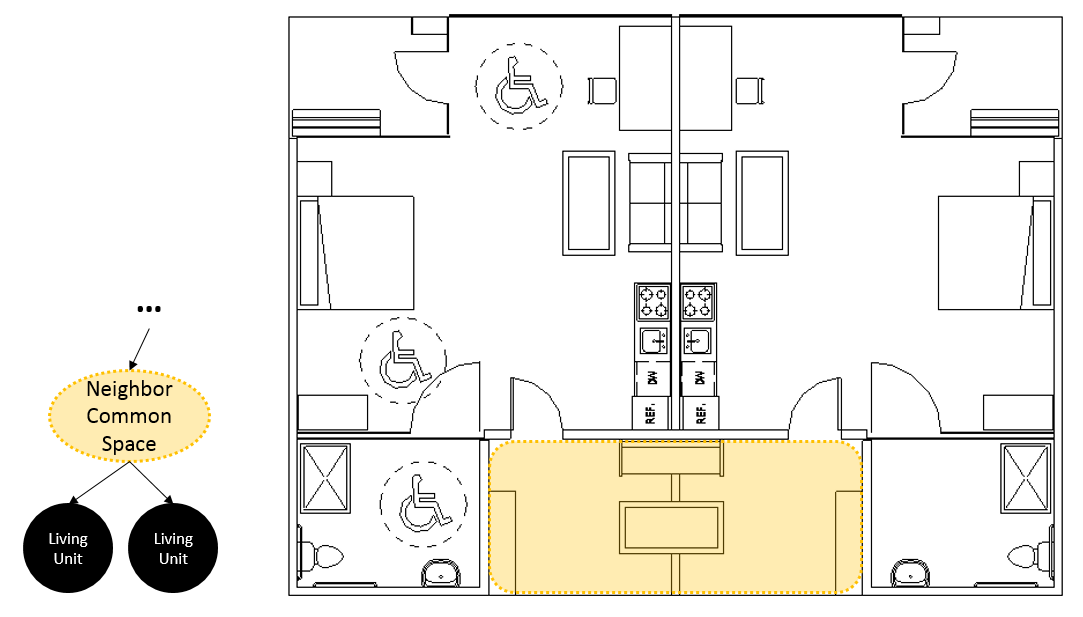
\includegraphics[width=\linewidth]{twoUnit-1.png}
  \caption{Common Space of Two Unit: Common Entrance}
  \label{fig:twoUnit-1}
\end{subfigure}
\begin{subfigure}{\textwidth}
  \centering
  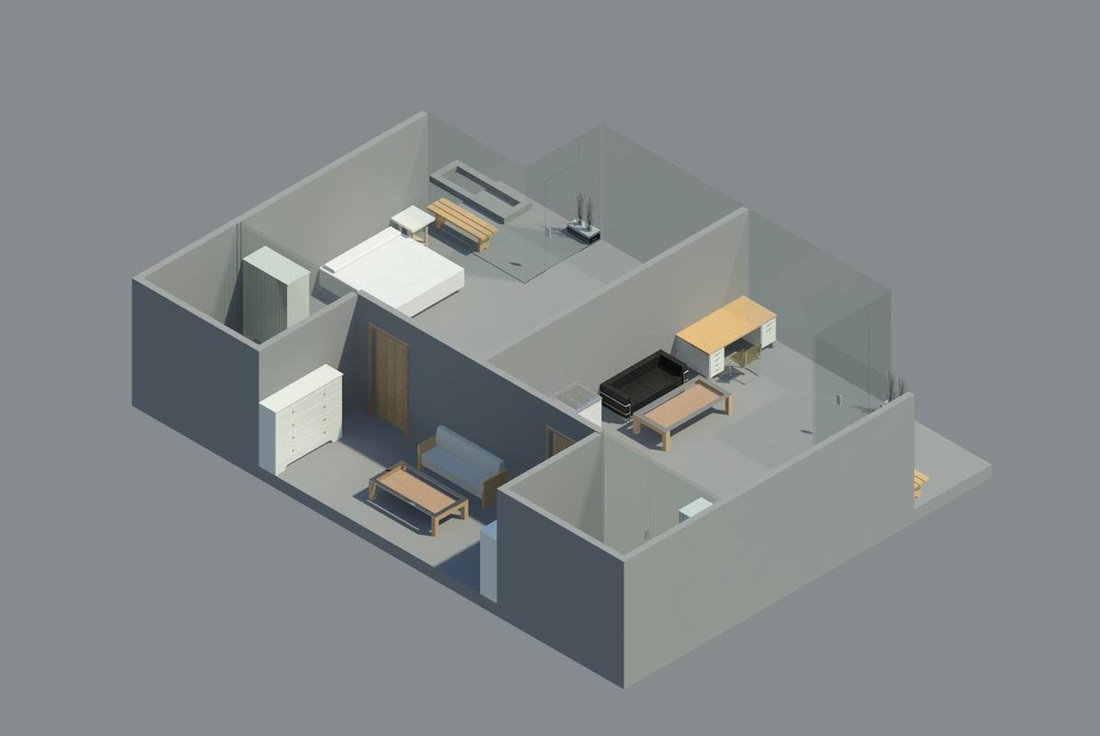
\includegraphics[width=\linewidth]{twoUnit-entrance.jpg}
  \caption{Perspective View of Common Space of Two Unit: Common Entrance}
  \label{fig:twoUnit-entrance}
\end{subfigure}
\caption{Two Unit Common Space}
\label{fig:twoUnitCommonSpaceEntrance}
\end{figure}

\clearpage
The balcony acts as another common space shared by
neighbors. Gardening activities can be undertaken at this
area. Although not exactly depicted in the plan, the garden space
should consider to be designed as raised garden to account for wheel
chair users (\fref{fig:twoUnitCommonSpaceGarden}).~
\begin{figure}[h!]
\centering
\begin{subfigure}{\textwidth}
  \centering
  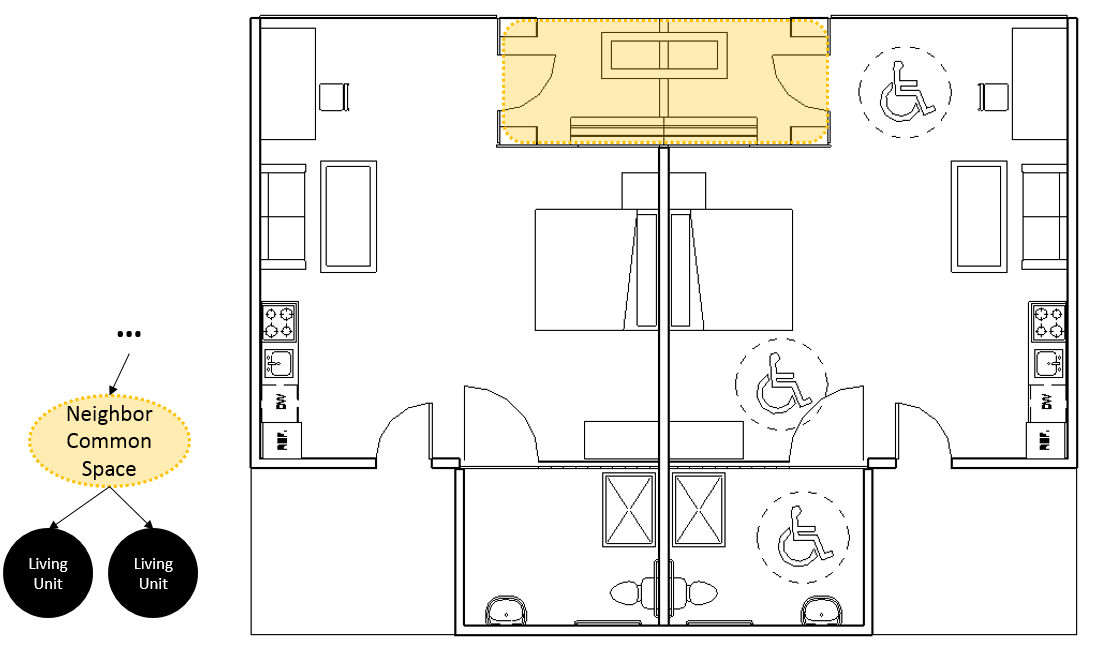
\includegraphics[width=\linewidth]{twoUnit-2.png}
  \caption{Common Space of Two Unit: Common Garden}
  \label{fig:twoUnit-2}
\end{subfigure}
\begin{subfigure}{\textwidth}
  \centering
  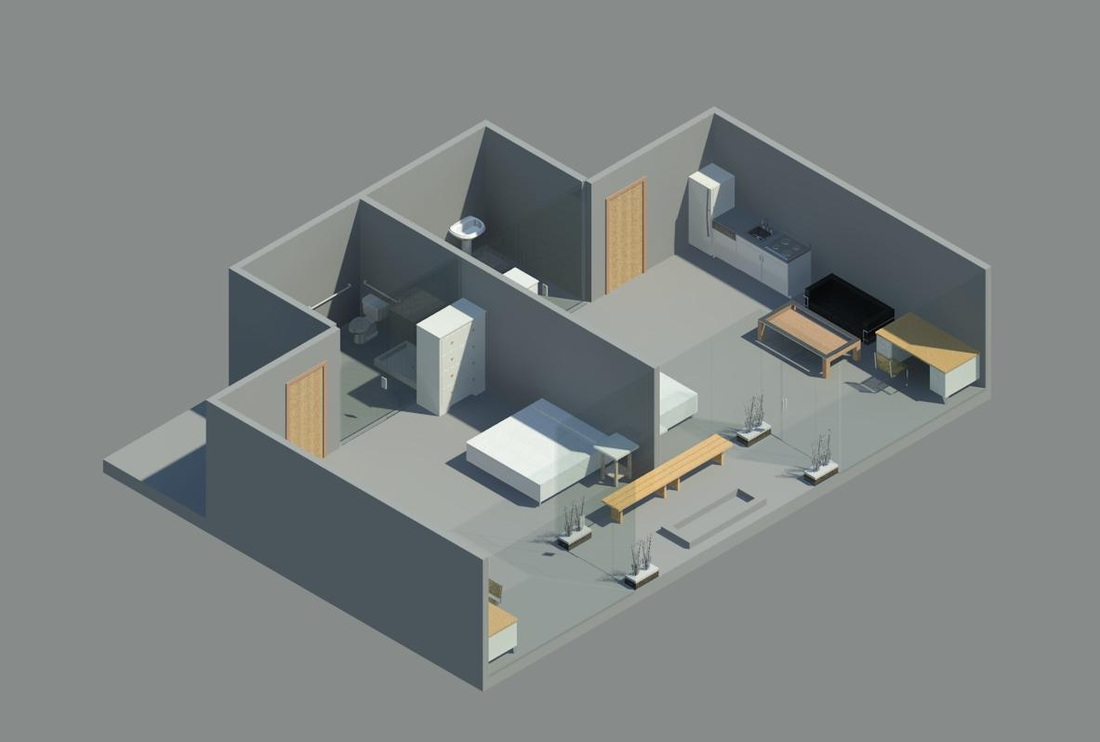
\includegraphics[width=\linewidth]{twoUnit-gd.jpg}
  \caption{Perspective View of Common Space of Two Unit: Common Garden}
  \label{fig:twoUnit-garden}
\end{subfigure}
\caption{Two Unit Common Space}
\label{fig:twoUnitCommonSpaceGarden}
\end{figure}

The common space of the eight unit shares the indoor garden on the
ground floor. The common space on upper floors shares the common view
to the lower floors.~
\begin{figure}
\centering
\begin{subfigure}{\textwidth}
  \centering
  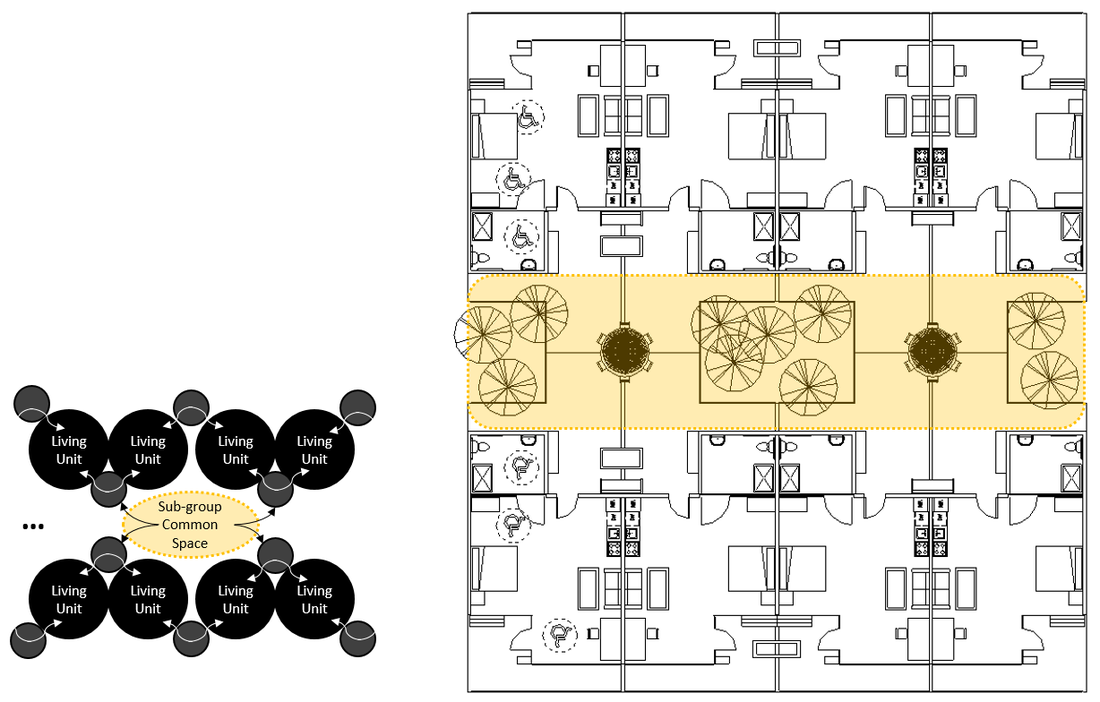
\includegraphics[width=\linewidth]{commonSpace8.png}
  \caption{Common Space of Eight Unit}
  \label{fig:commonSpace8}
\end{subfigure}
\begin{subfigure}{\textwidth}
  \centering
  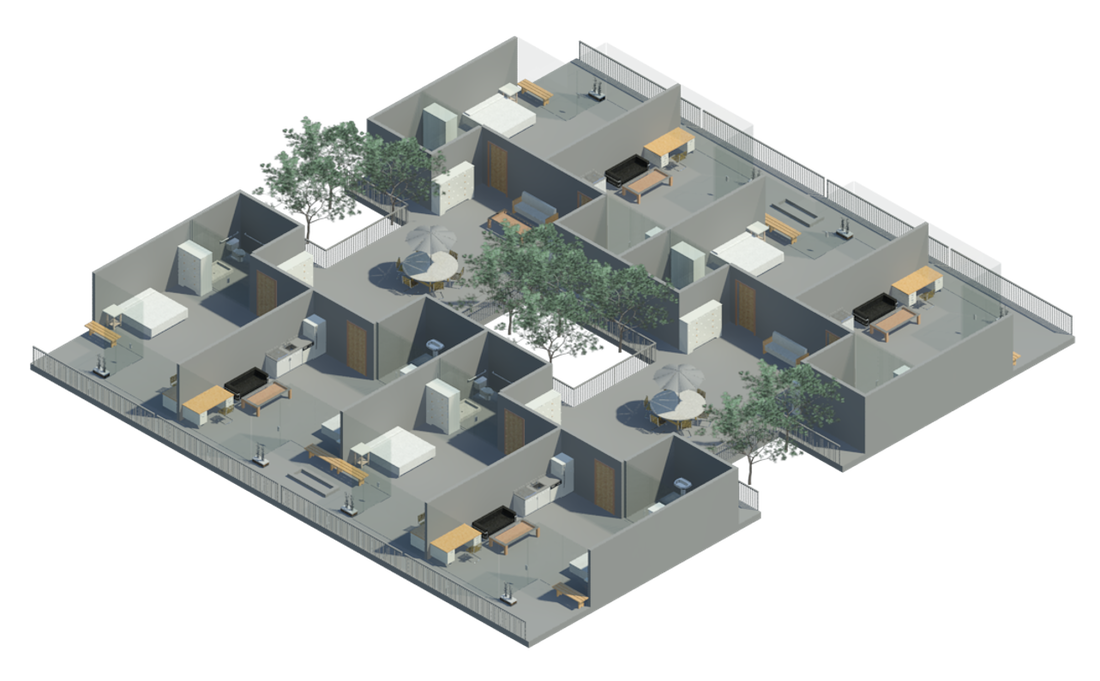
\includegraphics[width=\linewidth]{commonSpace8pers.png}
  \caption{Perspective View of Common Space of Eight Unit}
  \label{fig:commonSpace8pers}
\end{subfigure}
\caption{Eight Unit Common Space}
\label{fig:eightUnitCommonSpace}
\end{figure}
~
\begin{figure}
\centering
\begin{subfigure}{\textwidth}
  \centering
  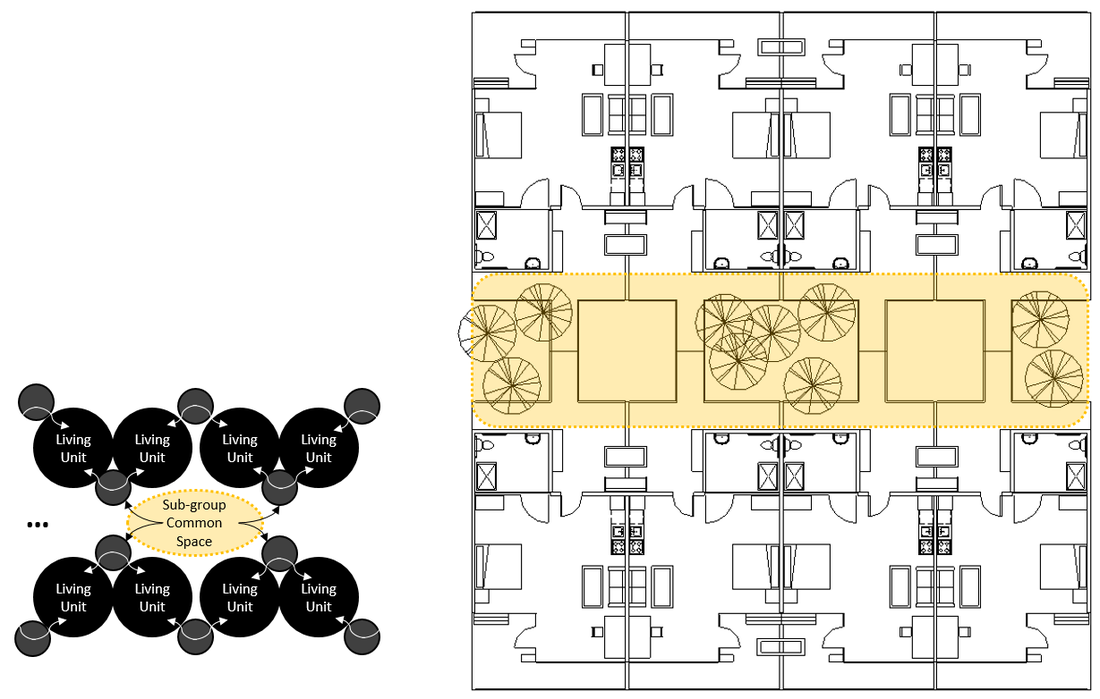
\includegraphics[width=\linewidth]{commonSpace8up.png}
  \caption{Common Space of Eight Unit: Upper Level}
  \label{fig:commonSpace8}
\end{subfigure}
\begin{subfigure}{\textwidth}
  \centering
  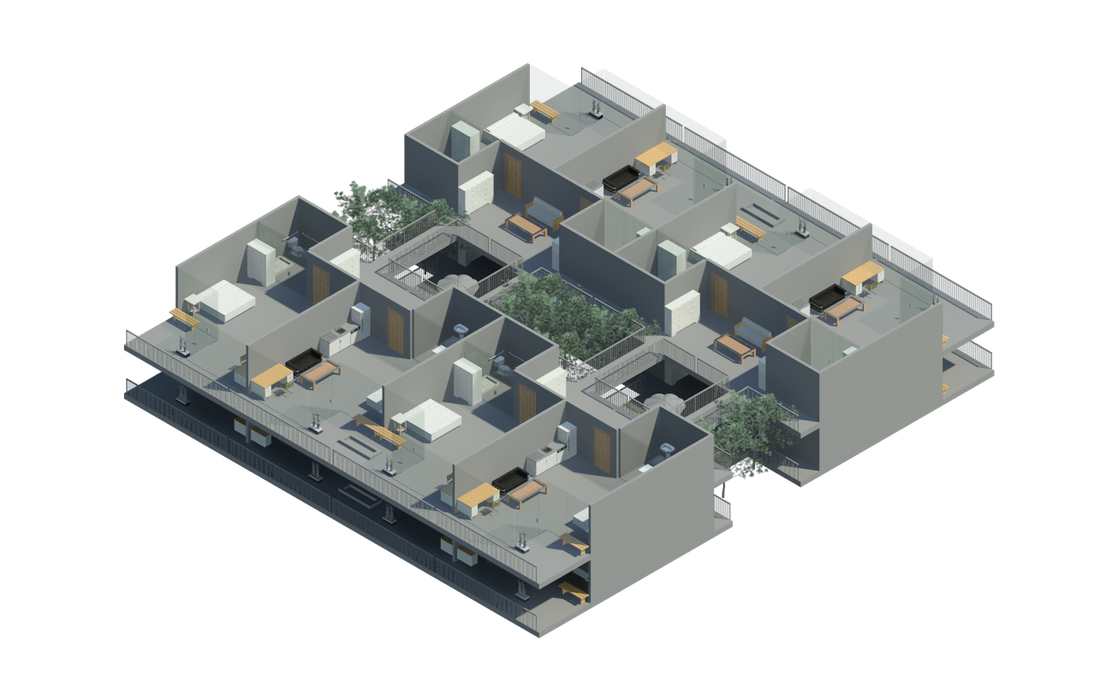
\includegraphics[width=\linewidth]{commonSpace8upPers.png}
  \caption{Perspective View of Common Space of Eight Unit: Upper Level}
  \label{fig:commonSpace8pers}
\end{subfigure}
\caption{Eight Unit Common Space: Upper Level}
\label{fig:eightUnitCommonSpaceUp}
\end{figure}

\clearpage
\section{Path Arrangement}~
The major concern for path design includes:
\begin{itemize}
\item To create more chance of encountering people, both the elderly
  residents and the young people.
\item To accommodate the needs for the Alzheimer Disease victims. \\A
  ``wandering loop'' (\fref{fig:path}) is needed to accomodate the
  behavior change for the Alzheimer Disease victims. For more detailed
  information, please refer to the case study in \cref{Chapter3}
\end{itemize}

\begin{figure}[htbp]
  \centering
  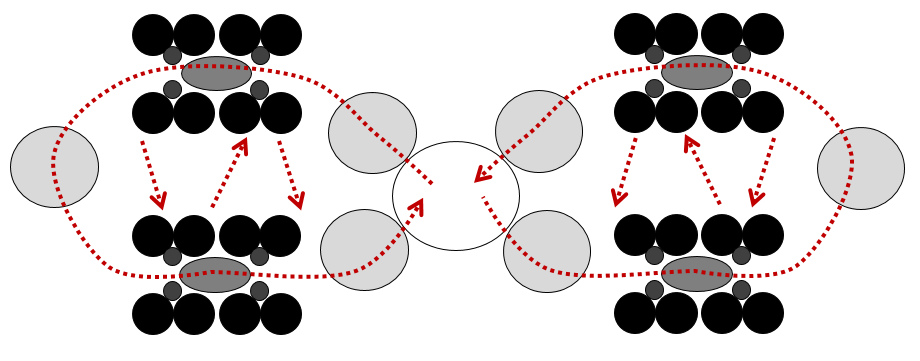
\includegraphics[width=0.7\textwidth]{path.png}
  \caption[Path Pattern]{Path Pattern}
  \label{fig:path}
\end{figure}

\subsection{Access to Nature}
In order to allow for easy access to nature, the indoor garden is
created between each of the two major row of living units, allowing
for access to nature in the indoor
environment~\fref{fig:indoorGarden}.
\begin{figure}[htbp]
  \centering
  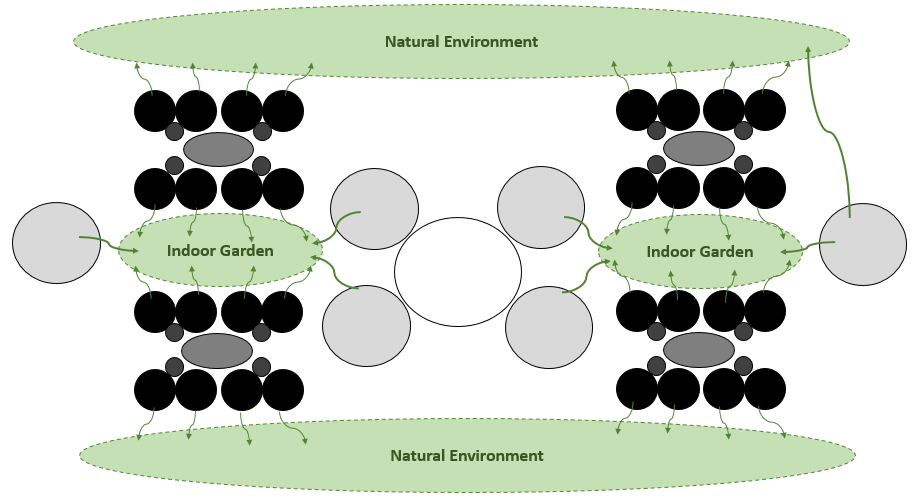
\includegraphics[width=0.7\textwidth]{indoorGarden.png}
  \caption[Access to Nature]{Access to Nature}
  \label{fig:indoorGarden}
\end{figure}
\section{Schematic for Sustainable System}
The components involved in the sustainable system include roof
gardens, rooftop pv system, green facade, rain collecting system and
food production chain resulted from the gardening. A draft system
integration diagram is shown in \fref{fig:sketchSustainable}
\begin{figure}[h!]
  \centering
  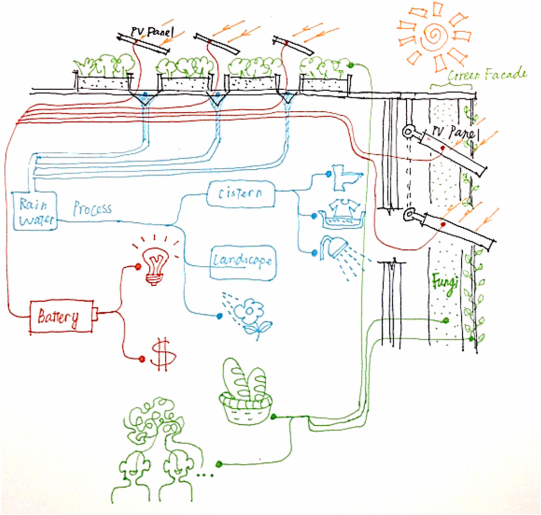
\includegraphics[width=0.8\textwidth]{sketchSustainable.png}
  \caption[System Integration Draft Diagram]{System Integration Draft
    Diagram}
  \label{fig:sketchSustainable}
\end{figure}